% Pregunta 3:
%\newpage
\textbf{(3pts.)} Muestra que la siguiente gram\'atica pertenece a la 
clase \textbf{LL(1)} pero no a la clase \textbf{SLR} ($E$ es el s\'imbolo inicial).
\[
E \to A \, a\, A\,b \;\mid\; B\,b\,B\,a \qquad \qquad  A \to \varepsilon 
\qquad\qquad B\to \varepsilon
\]

\textbf{Solución.} Para probar que la gramática dada (en adelante $G$) pertenece
a la clase $LL(1)$ y no a la clase $SLR$ basta con probar que $G \in LL(1)$, pues
$G$ tiene transiciones épsilon\footnote{De acuerdo a la definición: ``Una gramática
\textbf{LL} sin transiciones épsilon es una gramática \textbf{SLR}''.}. \newline

Ahora procedamos por contradicción, supongamos que $G \notin LL(1)$. Así, si encontramos
la tabla $LL(1)$ habremos acabado\footnote{Es fácil verificar que se cumplen las propiedes necesarias,
teniendo la tabla.}, pues es claro que $G$ no es recursiva por la izquierda.
Entonces,
\[
(1) E \to A \, a\, A\,b \;\mid\; B\,b\,B\,a \qquad \qquad  (2) A \to \varepsilon 
\qquad\qquad (3) B\to \varepsilon
\]
\begin{eqnarray*}
FIRST(E) = \{\epsilon\} &\qquad \qquad& FOLLOW(E) = \{\#\}\\
FIRST(A) = \{\epsilon\} &\qquad \qquad& FOLLOW(A) = \{a, b\}\\
FIRST(B) = \{\epsilon\} &\qquad \qquad& FOLLOW(B) = \{b, a\}
\end{eqnarray*}
Entonces, la tabla $LL(1)$ se ve de la siguiente manera:
\begin{center}
        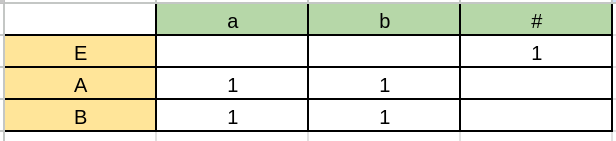
\includegraphics[scale=0.40]{./LL1.png}\\[0.4cm]
\end{center}
donde cada entrada registrada en la tabla fue consecuencia de tener
conjuntos $FIRST$ con un único elemento igual a $\epsilon$. Así, podemos
notar que cada entrada en la tabla obedece a un solo valor y por lo
tanto hemos podido construir nuestra tabla $LL1$, he aquí una contradicción
al suponer que $G \notin LL1$ y concluimos que $G \in LL1$. Además, como
las $\epsilon$-transiciones generaron nuestras entradas en la tabla, tenemos
que $G \notin SLR$.
